%-------------------------------------------------------------------------------
%
% TUM Dissertation Template
%
% For usage instructions see README.md
%
% Authors:
%   Andre Richter, andre.richter@tum.de
%   Michael Vonbun, michael.vonbun@tum.de
%   Christian Herber, christian.herber@tum.de
%   Stefan Wallentowitz, stefan.wallentowitz@tum.de
%
%-------------------------------------------------------------------------------
\documentclass[%
  % layouttitlepage,            % layout help rules (to see if you need
  %                             % some extra vspace in your title etc.)
  % headings = standardclasses, % serif fonts for headings
  % headings = big,             % If you use serif fonts for headings (above option
  %                             % uncommmented), uncomment this one to get smaller
  %                             % headings
  % sansseriftitlepage,         % sans serif title page
  % notocintoc,                 % do not add toc to toc itself
]{tumDiss}
\usepackage[utf8]{inputenc}
\usepackage{svg}


%-------------------------------------------------------------------------------
% Binding correction for the title page.
% WARNING: ONLY NEEDED FOR THE PRINT VERSION!
%
% After printing and binding, the left part of the titlepage may lose
% significant space, for example due to overlap from glue binding.
% You can increase the left margin of the title page with this option.
% This value of 8mm was measured for glue binding a thesis that was printed by
% the TUM Fachschaft EI and ~140 pages.
%-------------------------------------------------------------------------------
% \titlepagebindingcor{8mm}

%-------------------------------------------------------------------------------
% Binding correction for everything else.
% Does not affect titlePageBindingCor!
%
% WARNING: THIS OPTION CAN SHAKE UP YOUR CURRENT LAYOUT.
% If you want to use it, it is best to work with it from the very start. Adding
% it when finishing your dissertation might get you into trouble.
%
% Search http://texdoc.net/texmf-dist/doc/latex/koma-script/scrguien.pdf for
% "BCOR" for further reading.
%-------------------------------------------------------------------------------
% \KOMAoptions{BCOR=3mm}



%-------------------------------------------------------------------------------
% Faculty
%-------------------------------------------------------------------------------
\faculty{Fakultät für Informatik}

%-------------------------------------------------------------------------------
% Degree
%-------------------------------------------------------------------------------
\degree{PhD (check specific degree))}

%-------------------------------------------------------------------------------
% Title
%
% IMPORTANT:
%
% You must add manual line breaks here. If you don't, you'll get uneven spacing
% between the lines.
% YOU ALSO NEED THE BREAK AT THE LAST LINE.
%-------------------------------------------------------------------------------
\title{%
  Integration of Mixed-Criticality into Dynamic Task Migration for Real-Time Embedded Systems
}
% \subtitle{That is extended by using an additional subtitle}

%-------------------------------------------------------------------------------
% People
%-------------------------------------------------------------------------------
\author{Octavio Ivan Delgadillo Ruiz}
\vorsitz{Prof. Dr. Uwe Baumgarten}
\erstpruef{Prof. Dr.-Ing. Vorname Nachname}

% Use this one for a TUM professor
\zweitpruef{Prof. Dr.-Ing. Vorname Nachname}

% Or this one for an external professor
%\zweitpruef[Technische Universität Berlin]{Prof. Dr.-Ing. Vorname Nachname}

% Optionally, add a third examiner
%\drittpruef[RWTH Aachen]{Prof. Dr.-Ing. Max Mustermann}

%-------------------------------------------------------------------------------
% Hand in date
%
% This is the date of your personal hand-in at the TUM doctoral office.
%-------------------------------------------------------------------------------
\date{01.01.2016}

%-------------------------------------------------------------------------------
% Accepted date
%
% You can set this after your thesis was accepted. For handing in,
% it is not needed (at least for the Electrical Engineering faculty).
%-------------------------------------------------------------------------------
\dateaccepted{10.05.2016}



%-------------------------------------------------------------------------------
% Change language, e.g. to german
%-------------------------------------------------------------------------------
% \usepackage[ngerman]{babel}

%-------------------------------------------------------------------------------
% Compatibility issues
%-------------------------------------------------------------------------------
% If you need pstricks, load it here before everything else.
% Otherwise, tikz patterns won't work
%\usepackage{pstricks}

%-------------------------------------------------------------------------------
% Suggested standard packets are included here
%-------------------------------------------------------------------------------
% Loading scrhack fixes:
%   (1) KOMA-Script incompatible macros used in listings package.
%   (2) Inconsistent anchors in hyperref.
\usepackage{scrhack}


% figure inclusion
\usepackage[
  caption = false,
  font    = footnotesize
]{subfig}
\usepackage{graphicx}
\usepackage{pgfplots}
\usepackage{pgfplotstable}
\tikzset{>=stealth}
\usetikzlibrary{patterns}
\usetikzlibrary{pgfplots.statistics}
\usepackage[%
	backend=bibtex,
	url=false,
	style=alphabetic,
	maxnames=4,
	minnames=3,
	maxbibnames=99,
	giveninits,
	uniquename=init]{biblatex} % TODO: adapt citation style
% code block insertion
\usepackage{moreverb}
\usepackage{listings}

% math and equations
\usepackage{amsmath}
\usepackage{amssymb}
\usepackage{amsfonts}
\usepackage{upgreek}

% enumeration
\usepackage{enumerate}

% Source code with highlighting
\usepackage{listings}
\lstset{
  basicstyle       = \footnotesize,
  captionpos       = b,
  tabsize          = 4,
  commentstyle     = \color{TUMGreen},
  keywordstyle     = \color{TUMBlue},
  stringstyle      = \color{TUMOrange},
  otherkeywords    = {
    uint64_t,
    uint32_t,
    uint16_t,Poccistraße, Múnich-Ludwigsvorstadt-Isarvorstadt
    uint8_t,
    u64,
    u32,
    u16,
    u8,
    inline
  },
  numbers          = left,
  xleftmargin      = 7ex,
  aboveskip        = 4ex,
  abovecaptionskip = 2ex,
}

% Support for siunitx
\usepackage{siunitx}
\sisetup{
  exponent-product = \cdot,
  output-product   = \cdot,
  per-mode         = symbol-or-fraction,
  quotient-mode    = fraction,
  binary-units     = true
}

% No widows and orphans
\usepackage[all]{nowidow}

% dummy text
\usepackage{lipsum}

% hyperlinks
% according to its documentation, hyperref should be loaded last
% a list of packages that should be loaded after hyperref can be found at
% https://tex.stackexchange.com/questions/1863/which-packages-should-be-loaded-after-hyperref-instead-of-before
\usepackage{url}
\usepackage[
  hidelinks,
  bookmarksnumbered
]{hyperref}

% If hyperref is used, references to tables and figures link to their captions
% and not the actual tables or figures. This is especially unwanted for figures,
% because their captions are below the figure so that clicking on a link just
% shows the captions and the figure is invisible.
%
% Using the caption package fixes this behaviour.
\usepackage{caption}

% glossary functionality
% loading glossaries after hyperref adds hyperlings to acronyms and glossary
% entries
\usepackage[
  toc,
  acronym,
  style = long
]{glossaries}
\makeglossaries

%-------------------------------------------------------------------------------
% Include custom packages here
%-------------------------------------------------------------------------------

% \usepackage{}


%-------------------------------------------------------------------------------
% TUM CI colors for PGF
%-------------------------------------------------------------------------------
\definecolor{grey60} {RGB} {102, 102, 102} % 60% grey

%-------------------------------------------------------------------------------
% Default values for pgfplots
%-------------------------------------------------------------------------------
\newcommand{\figureHeight}{0.5625} %% 16:9
\pgfplotsset{
  compat           = 1.13,
  grid             = major,
  enlarge x limits = 0,
  cycle list name  = tum,
  major grid style = {dotted},
  minor grid style = {dotted},
  legend style     = {
    at     = {(0.98,0.96)},
    anchor = north east,
  },
  width            = \hsize * 0.9,
  height           = \hsize * 0.9 * \figureHeight,
}

%-------------------------------------------------------------------------------
% Correct bad hyphenation here
%-------------------------------------------------------------------------------
\hyphenation{op-tical net-works semi-conduc-tor}

%-------------------------------------------------------------------------------
% Acronyms (will be sorted alphabetically)
%-------------------------------------------------------------------------------
\newacronym{cpu}{CPU}{Central Processing Unit}
\glsadd{cpu}

\newacronym{pci}{PCI}{Peripheral Component Interconnect}
\glsadd{pci}

\newacronym{pcie}{PCIe}{Peripheral Component Interconnect Express}
\glsadd{pcie}

\newacronym{mmu}{MMU}{Memory Management Unit}
\glsadd{mmu}



%-------------------------------------------------------------------------------
% Actual document starts here
%-------------------------------------------------------------------------------
\begin{document}
\frontmatter
\maketitle

%-------------------------------------------------------------------------------
\chapter{Abstract}

\lipsum[1-4]



%-------------------------------------------------------------------------------
\chapter{Zusammenfassung}

\lipsum[1-4]



%-------------------------------------------------------------------------------
\tableofcontents
\listoffigures
\listoftables
\printglossary[type=\acronymtype, nonumberlist]



%-------------------------------------------------------------------------------
\mainmatter

% !TeX root = ../main.tex
% Add the above to each chapter to make compiling the PDF easier in some editors.

\chapter{Introduction}\label{chap:introduction}

**** FIX BIBLIOGRAPHY, not loading for some reason *****

Trends in the automotive industry are shaping the future of cars in a way that electronic and computing devices are becoming increasingly important. In fact, the majority of innovations in the automotive sector are related to electronic systems, either in the form of hardware or software~\parencite{ey1}. Developments such as vehicle electrification, autonomous driving and vehicle connectivity are only some examples of automotive applications where computer processing has a big relevance~\parencite{pwc1}. It is therefore reasonable to seek for approaches to ensure their usage is efficient and safety requirements are met.

In modern cars, dozens of computers, commonly known as electronic control units (ECUs), execute the various computing tasks present in a car. This number is likely to increase if we consider past trends: as the tasks performed by ECUs often have safety-critical constraints, such as real-time capabilities, they are commonly integrated to serve a specific purpose, avoiding conflicts caused by the parallel execution of other tasks~\parencite{vipin1, vipin2}. However, this strategy has shortcomings in the form of inefficient usage of the electronic devices (many tasks are only executed in specific and rare situations), reduced fault tolerance if a system fails, and increased weight and cost of the vehicle due to the high number of ECUs and cables~\parencite{vipin2, baunach1}. Hence, it is an important topic in the automotive industry to find solutions for these issues, especially optimizing costs, while ensuring vehicle safety is kept~\parencite{mckinsey1}.

ECU consolidation is an approach for the reduction in the number of electronic devices in the car. The idea is to consolidate the execution of the tasks from many single-purpose ECUs to a few powerful, multi-purpose ECUs. However, the implementation of ECU consolidation raises other challenges: as more tasks need to be executed on the same platform, higher computation and safety requirements must be met. Regarding safety, it is important to consider the added complexity, and cases where a hardware or software failure occur need to be considered, since a single failure could block many tasks and cause major issues. Also, some safety-critical tasks require redundancy to ensure their correct execution~\parencite{mundhenk1}. These challenges have motivated previous research at the chair of operating systems of the Technical University of Munich, where research on projects such as KIA4SM and MaLSAMi has explored the concept of dynamic task migration as a process where the execution of any tasks could move at any given time from one ECU to another. This would allow tasks to finish execution in case an ECU is overloaded or stops working, effectively allowing them to finish executing and meet their real-time constraints.

Previous work at the chair has divided the task migration process in two stages: planning and execution. The planning is the stage which generates a task distribution to the devices that will execute them. The execution is then responsible for allowing tasks to migrate from one device to another, while ensuring their progress is not lost and the execution continues and finishes correctly at the target device. So far, the work performed at the chair has explored the approach with a single criticality level, using different priority strategies for scheduling the tasks on an ECU (that is, deciding which task should get the processor and be executed at a given time). While this idea is in itself an important contribution, it is relevant to note that in many safety-critical embedded applications, such as the aerospace and automotive industries, different criticality levels exist, which are often defined in standards such as the ISO 26262, which defines the ASIL (automotive safety integrity level). For example, in a car, the correct functioning of the ABS is highly critical, as a failure could be fatal. In contrast, the functionality of the radio system has a lower criticality, as an eventual failure would not cause any issue other than an unpleasant trip. This idea is also important because in these industries there exist certification agencies that validate a system before it can be distributed.

For this reason, and due to the relevance of the concept of mixed-criticality in many industries, it would be important to expand the research on task migration to explore its integration. In particular, expanding the execution stage to ensure tasks with higher criticality are always able to execute properly and meet their deadline is crucial. But also it is important to find a balance between resource efficiency and reliability of the migration process for different criticality levels. Therefore, the work proposed as part of this PhD program aims to implement a strategy for the migration execution at different levels of criticality. Additionally, the mixed-criticality concept has to be integrated as well into the planning stage. This will be also explored in the scope of this research, although the main focus will be in the execution stage.

Furthermore, another important trend is the integration of edge technologies (known as multiaccess edge cloud or mobile edge computing - MEC - or in the specific automotive use-case vehicular edge cloud - VEC- ) for augmenting the vehicle's capabilities in aspects such as communication with other traffic participants or information services, increased sensing capabilities, offloading of tasks, etc (add reference). In the scope of this dissertation, it is considered that edge computing resources can be used to provide a further execution possibility for non-critical tasks under 2 circumstances: 1) the task would benefit from the availability of more powerful computing resources and sensing inputs, and 2) the physical hardware is at a critically high task load level and low criticality tasks would otherwise starve. It is considered that for the most highly critical tasks (like the ones interacting directly with the control of actuators like steering or vehicle speed) this approach is not feasible, as communication with an external component is always prone to interruption, even with the low latencies provided by new communication technologies such as 6G or 5G (add ref).

Although the work performed as part of this research is based on previous developments at the chair and will likely extend existent tools, it includes the development of a platform that implements mixed-criticality scheduling, as well as a migration system that involves the concept in different areas in the planning and execution stages. This includes the selection of hardware and software, as well as network interfaces. Also, verification of the algorithms used will be performed to ensure safety and timing requirements are met.

\section*{Research Questions}
To better define the scope and goal of the research performed in this thesis, following research questions have been propsed as basis (*** Maybe remove and integrate better into Intro text****):

\begin{itemize}
	\item 1. To what extent is task migration feasible in such a distributed real-time system while respecting real-time constraints, and under what conditions?
	\item 2. Given the system's need to handle uncertainty and adapt to changes in hardware availability and task load, how should tasks be prioritized based on criticality? 
	\item 3. What migration approaches - both at communication level and at OS level - are most suitable for high- and low-criticality tasks considering a trade-off between minimizing downtime and optimizing resources?
	\item 4. How feasible is extending the system by offloading tasks to virtual edge resources? What are the implications of this approach, especially in terms of latency, response time, safety and resource optimization?
\end{itemize}

---- See how to integrate into text but:
Following chapters / aspects help find an answer to the research questions:
Q 1: ...
Q 2: Approach, Base OS
Q 3: Migration,  
Q 4: Base OS, Results

\section*{Related Work}\label{section:relatedwork}
At the chair, previous research projects, such as KIA4SM and MaLSAMi, have explored the possibility of migrating tasks running on a device to another in a real-time capable system (for example, ECUs in a vehicle) under certain conditions. As mentioned before, in these works, the migration was divided into two main stages: The first is the migration planning, which determines the hardware that tasks will be migrated to, should the original hardware not be able to fulfill its duty (for example, if there is a failure in that hardware or if the real-time constraints or deadlines would be violated). The second is the execution of the migration, which ensures that corresponding tasks can be migrated from the source device to the target device while keeping their current state.

The migration execution has been explored previously at the chair, for example in projects KIA4SM and HaCRoM. This was explored in the form of a real-time checkpoint-restore mechanism. This involves creating and storing a snapshot of running tasks in a shared memory or copying the memory from a device to another. The work is based on Fiasco.OC and Genode OS. 

MaLSAMi and subsequent theses analyzed migration planning, with researchers performing schedulability analysis based on machine learning (specifically, on neural networks). Machine learning was picked over traditional mathematical approaches such as the ones proposed by Buttazzo~\parencite{buttazzo1}, because the recurrent calculations can become too complex for complex tasks and for big task sets, and they often lead to a pessimistic calculation of the system utilization. By predicting the feasibility of a task set using machine learning algorithms, potentially faster but less precise results are obtained, as demonstrated by previous theses by Taieb~\parencite{taieb1}, Utz~\parencite{utz1} and Blieninger~\parencite{blieninger1}. The predictions provided by the machine-learning approach indicate whether a task set is 100\% schedulable or not, but they are not completely safe, since false positive predictions may occur. This approach could be a potentially powerful solution for enabling the execution at run-time of the real-time capable migration planning. 

Additionally, a few different platforms and setups have been explored in these projects. The used operating systems running on the ECUs are Genode OS, as used in MaLSAMi and a few theses, a real-time operating system based on an extension of Genode OS with Fiasco.OC, as used in KIA4SM~\parencite{kia1} and HaCRoM, and FreeRTOS, as used by Delgadillo~\parencite{delgadillo1}. These developments are considered in the selection of the platform.

These projects have achieved research-relevant results in their segments, but the concept of mixed-criticality has not been explored in related chair internal work. It is therefore necessary to look at relevant chair-external work. In particular, those regarding mixed-criticality scheduling strategies and related to task migration are reviewed next.

It is worth noting that to my knowledge, research on mixed-criticality task migration of high criticality tasks, especially applied to the idea of ECU consolidation, has not been published. A possible reason for the lack of research in this area is the fact that nowadays safety is valued much higher than resource efficiency, thus overseeing the potential for optimization in this aspect. However, in my opinion, it should be possible to achieve both goals by implementing a holistic strategy and therefore it is an area where research can contribute importantly.





\chapter{State of the Art}
\label{chap:sota}

Example citations~\cite{barham2003xen, LIS}.
Example acronym usage \gls{cpu}.



% !TeX root = ../main.tex
% Add the above to each chapter to make compiling the PDF easier in some editors.

\chapter{Approach}\label{chap:approach}

The proposed system is a "breathable" distributed system, where breathable means that it can react at runtime to distinct situations to reconfigure itself and update a decision of where the tasks will execute, always prioritizing the execution of tasks based on their criticality. The situations that trigger this breathable behavior are mainly categorized in two types: 1) changes to the set of tasks that the system must execute (task queue) and 2) changes to the availability of computing resources. In the first category, it is assumed that all tasks have at least soft real-time behavior and they can all be categorized as periodic (need to be executed every certain time and constantly), sporadic (are executed upon request and only once) or a combination of both (might be triggered at a certain point in time and execute for a certain number of times with a period before finishing the processing) [**find a reference to support this assumption**]. The second category includes reacting to addition or removal of physical devices or hardware (for example, due to hardware failure or device restarts triggered by updates, etc.) and also to the availability and latency of virtual devices in the mobile-edge-cloud (for example, when driving over a highway section with MEC support).

These characteristics of the system can be summarized in the image below (add proper reference). The system behavior can be then described as follows. First, a reconfiguring situation triggers a re-distribution of the tasks that need to be executed, which are kept in the global queue. This global task queue as well as the set of both physical and virtual devices (or ECUs) are fed to a task partitioning algorithm, which decides a task-to-board mapping and then triggers the distribution of the tasks on the respective mapped device. The final step is that, depending on the previous mapping of tasks to boards, if the assigned ECU for a task changes, it is necessary to migrate its execution from the previous device (source) to the new one (target). This last step is the main objective of this research work, and in the scope of it, a few requirements should be considered to deem the implementation as successful: 1) the task has to be stopped in the source device and started in the target device, 2) the relevant task context should be also migrated, meaning that no crucial data is lost (in the case of a SLAM algorithm, the map and position would not be lost), 3) both the migration decision and execution strategies should consider the criticality of the tasks, 4) real-time behavior should be also considered in the migration strategy. It is relevant to mention that a master ECU would be responsible for both keeping the global task queue, triggering the task-to-board distribution algorithm (which itself can run on a separate ECU or a specialized ML hardware) and keeping the relevant files to start tasks when necessary.
 

\begin{center}
	\makebox[\textwidth]{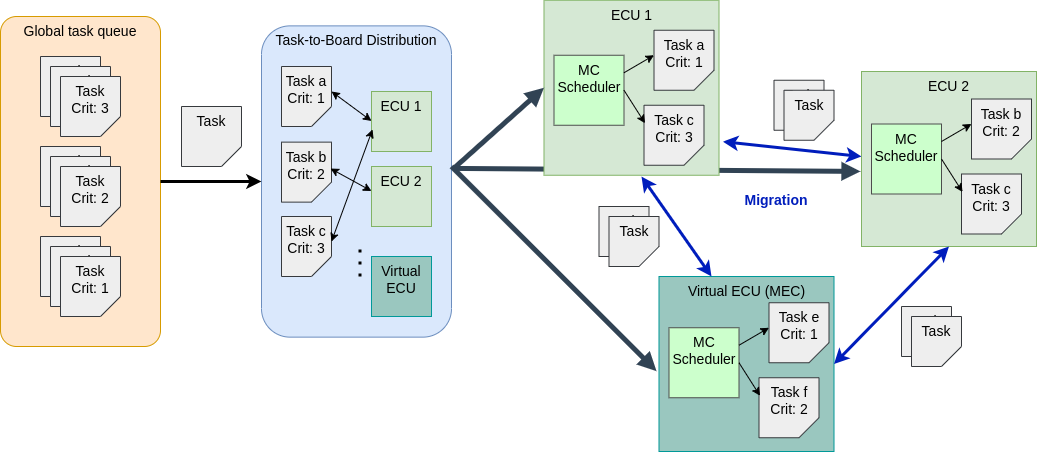
\includegraphics[width=\textwidth]{figures/Migration_Diag_new.png}}
\end{center}

Based on the previous list of requirements, and especially 3 and 4, at least 2 migration strategies should be implemented, since tasks with different criticalities also have different constraints to be prioritized. For example, in the case of low-criticality tasks, it might be more relevant that the task does not end in starvation, whereas for a high critical task it is crucial that the result is delivered always on-time and that, if the task needs to be paused due to a critical failure, it is brought back up in a reduced and deterministic time to keep up with the real-time constraints.



\section{Overview of the Approach}\label{section:descriptionapproach}

As mentioned before, the main objective of the proposed research is to achieve the integration of mixed criticality into the task migration process. The proper integration would require different strategies for the different criticality modes. For this reason, it is first important to define what is understood under mixed criticality in the scope of this work. While many publications consider only two criticality levels (high and low), the standards commonly describe several of them. In this work, the concept of multiple criticality levels will be used in a conceptual phase following the ASIL standard in ISO 26262, while the implementation and results will be collected for at least 2 levels in both the scheduling algorithm and the migration strategy. Whereas a model with multiple criticality levels represents real situations better over one with just two, as tasks can have intermediate criticality levels, in the scope of this work, the focus relies more on fulfilling challenges at both ends of the criticality spectrum, and assuming a mix of both strategies might apply as a solution for intermediate levels. One concept that should be covered is the consideration of different execution times according to a criticality level, as normally higher criticality levels offer pessimistic WCET estimates to ensure correct behavior occurs, but actual execution times are often lower. This is a concept that is explored in many publications and is often necessary to ensure compliance with certification authorities.

The first element needed for the system developed is the integration of a mixed-criticality scheduler for each of the physical devices. This should ensure that for any given device, the tasks with a higher criticality will never miss the deadline for a job, while being more flexible for lower criticality levels. In this regard, exploring different mixed-criticality scheduling algorithms and their integration in the development platform is an important step that will allow the migration to occur and be evaluated properly. Several publications have proposed mixed-criticality scheduling algorithms, such as ~\parencite{baruah1, fleming1, zhao1, baruah2, lili1}, and a few of them can be implemented and compared. It is also important to mention that following the state of the art in embedded devices, a multi-core implementation is desired, with asymmetrical multiprocessing (AMP) being the preferred solution, as software failures could be isolated to affect less tasks (***find a reference***). In particular, following approaches are explored (so far): hierarchical virtual deadline EDF (faulty implementation); reserved cores for 2-level MC, with LO crit cores as backup cores for HI tasks. It is assumed that this step should not affect the behavior of the virtual devices, since by concept, they can only run non highly (not necessarily only LO) critical tasks, due to the uncertainties introduced by the external communication with the MEC (explain further...).

Another important element for the distributed system to ensure its compliance to the real-time constraints is a timing protocol such as PTP, to keep the different devices synchronized and share the same notion of time when following task deadlines. This way, even when migrating a task, information on the deadlines should be very accurate. In addition to this, migration strategies must consider that transmission times can be variable and, in the ideal case, the source device should keep the original task execution until it is ensured that the target device has started the execution successfully, potentially taking longer than the deadline of a running job.

The migration planning will be adapted from previous work, namely the student theses supervised by Bernhard Blieninger. As these don't consider mixed-criticality or a multi-core implementation in the system behavior, a few changes are necessary to integrate both concepts. First, the schedulability analysis that is commonly used for selecting the best task distribution has to be extended to work with criticality levels and the use of a mixed-criticality scheduler. Here, it has to be taken into consideration whether extending and retraining the machine learning models is worth the effort, especially since this idea is still not proven as a solution and the extension with the criticality levels and other relevant information might add complexity to the net. Otherwise, implementing a mathematical schedulability analysis that considers mixed criticality is necessary. A second extension that should be performed in the planning stage is to penalize the migration of higher criticality tasks, as the migration overhead adds an additional risk for the tasks failing. Furthermore, the availability of both virtual and physical devices needs to be considered at the moment of deciding which tasks should migrate and where.

The next step in the development of this strategy is the execution of the migration, which is the core concept explored in this work. It is important to consider the necessity to meet strict timing constraints for tasks at the higher end of the criticality spectrum. ***THIS HI criticality solution is yet to be explored, Yinbo is working on the variant for LO crit*** While the exact approach is yet to be proven as feasible, an idea for higher criticality tasks would be to let them run in a standby state in all or a subset of the total of available ECUs, and only executing it in one ECU, while storing runtime generated data either in a central unit or in a shared memory only accessible to highly critical tasks, in this way only a start/stop signal is sent to the task and the execution can be resumed quickly, also ensuring fail-safety in case the executing device fails. Also, for tasks that require redundancy (e.g. ASIL level D), it should be possible for tasks to execute actively multiple times and produce results in parallel. Another addition in this stage should be the introduction of a real-time capable communication protocol. In this sense, it should be possible to bound the migration time for this tasks, ideally in the range of a few milliseconds. These ideas could be faster to execute and allow for less variance in the time, eventually making it possible to perform formal verification, but it would be expensive if tasks at all criticality levels were to run like that, as the resources are utilized inefficiently. This should be acceptable for highly critical tasks, though, since the majority of the tasks would be assigned low to medium criticality levels.

The strategy for migrating lower criticality tasks between physical devices is prone to more flexibility, so that a wider range of tasks can be deployed with a lower impact in terms of resource efficiency, even if this would open the possibility for more erroneous behavior in the tasks. The approach currently explored for tasks with low criticality involves the transmission of precompiled task binaries and a snapshot of the execution data every time a task is distributed to an ECU and the usage of a normal TCP/IP protocol over Ethernet. ***This is Yinbo's ELF loader thesis*** With this strategy, the resource utilization in the devices is made more efficient, but the time spent for the migration is increased as the communication is slower due to the amount of information exchanged, and also less reliable due to the nature of the communication protocol. 

As an optional step, the exploration of strategies for more criticality levels is yet to be done, but a few ideas are suggested. First, a combination of the two strategies mentioned could be implemented for intermediate criticality levels, such as leaving the tasks running but using a less predictable communication protocol. Another idea is to subdivide each of the criticality levels mentioned and there perform variations of the mentioned strategy. For example, in a system with a certain number of devices and 2 high criticality sublevels, the highest sublevel tasks are kept in standby on all devices, while the rest are only kept in standby in a few of the devices, making sure there is always an ECU ready for the highest criticality and using less resources for the second sublevel. In the case of lower criticality, this could be implemented in the form of giving priority to the migration and transmission of data of tasks at the higher sublevels.

Additionally, due to the consideration of virtual devices in the MEC, an additional strategy is also implemented in the scope of this work. That is, the migration of low criticality tasks from and to the MEC. For this implementation, it is assumed that the MEC servers share some aspects of the architecture with the real hardware and that the devices can be modeled in the form of containers as their digital twins. In this way, upon availability, the master ECU can request to start a container which will run the required task. It is assumed that this behavior is allowed for low criticality tasks that can benefit from the more powerful resources available in the MEC, and that communication latency can be neglected as long as the results produced are relevant. An example of this might be a path planning algorithm for an autonomous vehicle, where the immediate safety of the vehicle is not threatened, but the algorithm can be extended with further sensor data and better hardware for performing ML tasks. ***Part of this has already been implemented by Roberto*** It is relevant in the scope of the migration, that the virtual tasks have an equivalent task implemented for the real devices, and that the task data can also be migrated between them. In this way, the task can be moved depending on the need and availability of the resources to and from the MEC.



	


+
'
\chapter{Content}
\label{chap:content}

\lipsum[1]

\section{Example Section}

\lipsum[1-2]
\lipsum[66]



\subsection{Example Table}

\lipsum[1]

\begin{table}[thb]
    \renewcommand{\arraystretch}{1.3}
    \captionabove{Example Table.}
    \label{table:example_table}
    \centering

    \begin{tabular}{|r|l|}
      \hline
      7C0         & hexadecimal \\
      3700        & octal \\
      \cline{2-2}
      11111000000 & binary \\
      \hline
      \hline
      1984        & decimal \\
      \hline
    \end{tabular}
\end{table}


\lipsum[2-4]



\subsection{Example Plot}

\lipsum[1]

\begin{figure}[thb]
    \centering

    \begin{tikzpicture}
        \begin{loglogaxis}[
            xlabel={Degrees of freedom},
            ylabel={$L_2$ Error}
            ]
            \addplot coordinates {
              (5,8.312e-02)    (17,2.547e-02)   (49,7.407e-03)
              (129,2.102e-03)  (321,5.874e-04)  (769,1.623e-04)
              (1793,4.442e-05) (4097,1.207e-05) (9217,3.261e-06)
            };

            \addplot coordinates{
              (7,8.472e-02)    (31,3.044e-02)    (111,1.022e-02)
              (351,3.303e-03)  (1023,1.039e-03)  (2815,3.196e-04)
              (7423,9.658e-05) (18943,2.873e-05) (47103,8.437e-06)
            };

            \addplot coordinates{
              (9,7.881e-02)     (49,3.243e-02)    (209,1.232e-02)
              (769,4.454e-03)   (2561,1.551e-03)  (7937,5.236e-04)
              (23297,1.723e-04) (65537,5.545e-05) (178177,1.751e-05)
            };

            \addplot coordinates{
              (11,6.887e-02)    (71,3.177e-02)     (351,1.341e-02)
              (1471,5.334e-03)  (5503,2.027e-03)   (18943,7.415e-04)
              (61183,2.628e-04) (187903,9.063e-05) (553983,3.053e-05)
            };

            \addplot coordinates{
              (13,5.755e-02)     (97,2.925e-02)     (545,1.351e-02)
              (2561,5.842e-03)   (10625,2.397e-03)  (40193,9.414e-04)
              (141569,3.564e-04) (471041,1.308e-04) (1496065,4.670e-05)
            };

            \addplot coordinates{
              (15,6.75e-02)     (123,3.425e-02)     (745,1.751e-02)
              (5561,5.942e-03)   (30625,2.197e-03)  (90193,9.714e-04)
              (341569,3.564e-04) (871041,1.708e-04) (1896065,8.670e-05)
            };
            \legend{$d=2$,$d=3$,$d=4$,$d=5$,$d=6$,$d=7$}
        \end{loglogaxis}
    \end{tikzpicture}

    \caption{Example Plot.}

    \label{fig:example_plot}
\end{figure}

\lipsum[3]
\lipsum[66]



\subsection{Example Barchart}

\lipsum[1]

\begin{figure}[thb]
    \centering

    \begin{tikzpicture}
        \begin{axis}[
            ybar               = 5pt, % configures `bar shift'
            xmajorgrids        = false,
            x tick label style = {
              /pgf/number format/1000 sep =},
            xtick              = {1930, 1940, 1950},
            ylabel             = y-Axis,
            enlarge x limits   = 0.25,
            ymin               = 2e7,
            ymax               = 8e7,
            bar width          = 9pt,
            point meta         = y *10^-7, % the displayed number
            nodes near coords,
            ]
            \addplot
            coordinates {(1930,70e6) (1940,33e6)
              (1950,40e6)};

            \addplot
            coordinates {(1930,65e6) (1940,42e6)
              (1950,43e6)};

            \addplot
            coordinates {(1930,45e6) (1940,47e6)
              (1950,34e6)};

            \addplot
            coordinates {(1930,34e6) (1940,37e6)
              (1950,38e6)};

            \addplot
            coordinates {(1930,28e6) (1940,27e6)
              (1950,30e6)};

            \addplot
            coordinates {(1930,24e6) (1940,31e6)
              (1950,33e6)};

            \legend{One, Two, Three, Four, Five, Six}
        \end{axis}
    \end{tikzpicture}

    \caption{Example Barchart.}

    \label{fig:example_barchart}
\end{figure}

\lipsum[3]
\lipsum[66]



\subsection{Example SVG Graphics Input}

\lipsum[1]

\begin{figure}[thb]
  \centering
  %\includesvg{shapes}

  \caption{Example Shapes from an SVG.}
  \label{fig:example_svg}
\end{figure}

\lipsum[42]



\subsection{Example Source Code}

\lipsum[1]

\begin{lstlisting}[
    language = C,
    caption  = {Example Source Code},
    label    = {list:example_src}
]
#include <stdio.h>

void quick_sort (int *a, int n) {
    int i, j, p, t;
    if (n < 2)
        return;
    p = a[n / 2];
    for (i = 0, j = n - 1;; i++, j--) {
        while (a[i] < p)
            i++;
        while (p < a[j])
            j--;
        if (i >= j)
            break;
        t = a[i];
        a[i] = a[j];
        a[j] = t;
    }
    quick_sort(a, i);
    quick_sort(a + i, n - i);
}

/* main routine */
int main (void) {
    int a[] = {4, 65, 2, -31, 0, 99, 2, 83, 782, 1};
    int n = sizeof a / sizeof a[0];
    int i;
    for (i = 0; i < n; i++)
        printf("%d%s", a[i], i == n - 1 ? "\n" : " ");
    quick_sort(a, n);
    for (i = 0; i < n; i++)
        printf("%d%s", a[i], i == n - 1 ? "\n" : " ");
    return 0;
}
\end{lstlisting}



\subsection{Example Subsection}

\lipsum[1]



\subsubsection{Example SubSubSection}

\lipsum[9]



\subsubsection{Example SubSubSection}

\lipsum[10]



\chapter{Conclusion \& Outlook}
\label{chap:conclusion}

\lipsum[1-4]



%-------------------------------------------------------------------------------
% Bibliography
%-------------------------------------------------------------------------------
%\backmatter
% unsrturl-custom works only with hyperref loaded
% use other styles like unsrt when hyperref is not loaded

\printbibliography{}



%-------------------------------------------------------------------------------
% Appendix
%-------------------------------------------------------------------------------
\appendix
\chapter{Additional Stuff}

\lipsum[1-4]

\end{document}

%%% Local Variables:
%%% mode: latex
%%% TeX-master: t
%%% End:
